\clearpage
\begin{trapbox}
\textbf{易错点1：左右支把两个焦半径分配反了。}

\begin{center}
% C093：左右同尺度的错误/正确配对对照；几何长度始终为3和5。
% 公共点位于左支，F1=(0,0),F2=(4,0),P=(0,3) (局部平移坐标)
\begin{tikzpicture}[scale=0.82,>=stealth]
 \begin{scope}
  \coordinate (L) at (0,0); \coordinate (R) at (4,0); \coordinate (P) at (0,3);
  \draw[gray,thick] (L)--(R);
  \draw[teal!70!black,very thick] (L)--(P);
  \draw[orange!85!black,very thick] (R)--(P);
  \foreach \q/\loc/\t in {L/below/F_1,R/below/F_2,P/above/P}{\fill (\q) circle(1.8pt) node[\loc]{$\t$};}
  \node[red!75!black,above] at (2,3.65) {\textbf{错误：数值配反}};
  \node[red!75!black,left] at (-0.08,1.5) {$PF_1=5\;\times$};
  \node[red!75!black,above right] at (2.2,1.8) {$PF_2=3\;\times$};
  \node[below] at (2,-0.85) {$P$ 在左支，近 $F_1$};
 \end{scope}
 \begin{scope}[xshift=7cm]
  \coordinate (L) at (0,0); \coordinate (R) at (4,0); \coordinate (P) at (0,3);
  \draw[gray,thick] (L)--(R);
  \draw[teal!70!black,very thick] (L)--(P);
  \draw[orange!85!black,very thick] (R)--(P);
  \foreach \q/\loc/\t in {L/below/F_1,R/below/F_2,P/above/P}{\fill (\q) circle(1.8pt) node[\loc]{$\t$};}
  \node[teal!70!black,above] at (2,3.65) {\textbf{正确：按实际长度}};
  \node[teal!70!black,left] at (-0.08,1.5) {$PF_1=3$};
  \node[orange!85!black,above right] at (2.2,1.8) {$PF_2=5$};
  \node[below] at (2,-0.85) {$3^2-5^2<0$};
 \end{scope}
\end{tikzpicture}

\end{center}

左支的点离左焦点近，离右焦点远。
图中两幅三角形\emph{点的位置和实际长度相同}，
左图故意把 $3$、$5$ 标签写反，以便和右图逐一对照。
\[
\boxed{x_P<0\ \Longrightarrow\ PF_1<PF_2},\qquad
PF_1^2-PF_2^2=4cx_P<0.
\]
\textbf{正确替代：}先写无序的 $\{a+A,a-A\}$，
再看点在左支还是右支，最后决定哪段对应哪个焦点。
\end{trapbox}

\clearpage
\begin{trapbox}
\textbf{其他易错点：错误写法 $\to$ 错因 $\to$ 正确做法。}
\begin{itemize}
\item \textbf{漏掉绝对值：}误写
$PF_1-PF_2=2A$ 适用于所有公共点。
左支的差是负数；应写
$|PF_1-PF_2|=2A$，再按支别确定符号。
例如 $F_1=(-2,0),F_2=(2,0),P=(-2,3)$ 时，
$PF_1-PF_2=3-5=-2$。

\item \textbf{半轴混淆或再乘2：}若 $a=4,A=1$，
正确两长度为 $5,3$；写成 $10,6$ 是把已经求出的长度重复乘2。
必须区分 $a$ 与 $A$，共焦\emph{只表示焦点相同}。

\item \textbf{把两条曲线不同的点联立：}若一个点在椭圆、另一个点在双曲线，
不能把两个点各自满足的关系写成同一个方程组。
必须先确认是\emph{同一个公共点}、\emph{同一对焦点}。

\item \textbf{忽略参数范围：}写出 $a-A$ 前应核对
$a>c>A>0$；例如 $c=2,A=4$ 就不满足双曲线的焦距关系。
两条焦半径必须为正长度。
\end{itemize}
\end{trapbox}

\clearpage
\begin{trapbox}
\textbf{易错点：误以为上下对称也会交换两条焦半径。}

\begin{center}
% Four exact intersections for a=4, A=1, c=2: (+/-2,+/-3)
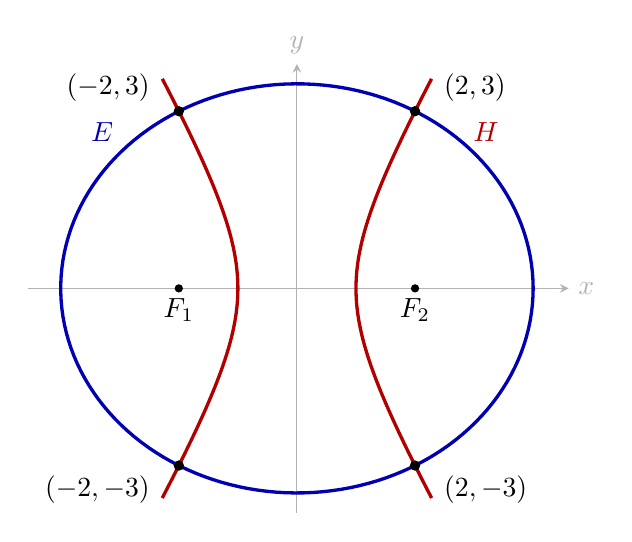
\begin{tikzpicture}[scale=0.75,>=stealth]
 \draw[->,gray!60] (-4.55,0)--(4.6,0) node[right]{$x$};
 \draw[->,gray!60] (0,-3.8)--(0,3.8) node[above]{$y$};
 \draw[blue!70!black,very thick,samples=160,domain=0:360,variable=\t]
  plot ({4*cos(\t)},{sqrt(12)*sin(\t)});
 \draw[red!70!black,very thick,samples=110,domain=-3.55:3.55,variable=\t]
  plot ({sqrt(1+\t*\t/3)},{\t});
 \draw[red!70!black,very thick,samples=110,domain=-3.55:3.55,variable=\t]
  plot ({-sqrt(1+\t*\t/3)},{\t});
 \foreach \x/\y in {2/3,2/-3,-2/3,-2/-3}{\fill[black] (\x,\y) circle (2.5pt);}
 \node[above right,xshift=7pt] at (2,3) {$(2,3)$};
 \node[below right,xshift=7pt] at (2,-3) {$(2,-3)$};
 \node[above left,xshift=-7pt] at (-2,3) {$(-2,3)$};
 \node[below left,xshift=-7pt] at (-2,-3) {$(-2,-3)$};
 \fill (-2,0) circle (2pt) node[below]{$F_1$};
 \fill (2,0) circle (2pt) node[below]{$F_2$};
 \node[blue!70!black] at (-3.3,2.65) {$E$};
 \node[red!70!black] at (3.2,2.65) {$H$};
\end{tikzpicture}

\end{center}

图中右侧 $(2,3)$ 与 $(2,-3)$ 关于 $x$ 轴对称，
到 $F_1$ 的距离同为 $5$，到 $F_2$ 的距离同为 $3$；
左侧两点则到 $F_1$ 同为 $3$、到 $F_2$ 同为 $5$。
\textbf{正确替代：}上下对称保持到每个焦点的距离；
只有左右对称才交换焦点对应。判长短看 $x_P$ 的正负。
\end{trapbox}

\clearpage
\begin{trapbox}
\textbf{三个15秒自测（可直接当课堂提问）。}
\begin{enumerate}
\item $a=6,A=2$，点在左支，求 $PF_1,PF_2$。
\textbf{答：}$PF_1=4,PF_2=8$。
\item $PF_1=8,PF_2=4$，反求 $a,A$。
\textbf{答：}$a=6,A=2$。
\item 焦距 $6$，椭圆半长轴 $5$、双曲线实半轴 $2$；
右支公共点到哪个焦点更近？
\textbf{答：}到右焦点 $F_2$ 更近，$PF_2=3$。
\end{enumerate}
\textbf{检查顺序：}共同焦点与同一个公共点 $\to$ 半轴范围
$\to$ 定和定差 $\to$ 左右支 $\to$ 正长度。
\end{trapbox}
